%% ID: roundabout
%% TITLE: Car on a Roundabout
%% TYPE: question
%% QUESTIONTYPE: symbolic
%% CONCEPTS: angular_circular, friction, resolving_vectors
%% VIDEOS: IntA1988PIIQ3l.mp4
%% LEVEL: 4
%% TOPIC: mechanics/circular
%% ORDER: 10
\begin{problem}[NHB_Roundabout]
{
\begin{enumerate}
\item A car approaches a roundabout of radius $R$. What is the maximum speed at which it can travel in order to go around without slipping, if the coefficient of friction between the road and car is $\mu$?
\item This time a racing car approaches a corner of radius $R$, banked at an angle $\theta$ to the horizontal. 
\begin{enumerate}
\item At what speed must the car travel if it is icy so there is no friction between the wheels and the road?
\item What is the maximum speed at which the car can travel and not slip if the road is rough, with coefficient of friction is $\mu$?
\item Is there a minimum speed at which the car needs to travel when the road is rough, with coefficient of friction $\mu$?\end{enumerate} \end{enumerate}} \answer{a. $v\le\sqrt{\mu gR}$, b.i) $v=\sqrt{gR\tan\theta}$, ii) $v\le\sqrt{\frac{\sin\theta+\mu \cos\theta}{\cos\theta-\mu \sin\theta}\cdot gR}$, iii) yes, $v\ge\sqrt{\frac{\sin\theta-\mu \cos\theta}{\cos\theta+\mu \sin\theta}\cdot gR}$}
{\textit{Created for the Rutherford School Physics Project by NHB and ES}}
{\begin{enumerate}
\item The forces acting on the car are shown in Figure \ref{fig:CircularMotion_c}.
\begin{figure}[h]
\centering
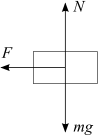
\includegraphics[width=3cm]{../../../figures/CircularMotion_c.eps}
\caption{}
\label{fig:CircularMotion_c}
\end{figure}
\\
The condition for circular motion is
\begin{equation*}
F=mv^2/R
\end{equation*}
since the frictional force $\vtr{F}$ is the only force acting in the horizontal direction. Resolving vertically gives
\begin{equation*}
N=mg
\end{equation*}
and we know that $F=\mu N$ on the point of slipping, therefore
\begin{equation*}
\mu N=\mu mg=mv^2/R
\end{equation*}
\begin{equation*}
\Rightarrow v^2=\mu gR
\end{equation*} therefore
\begin{equation*}
v\le\sqrt{\mu gR}
\end{equation*}
for the car not to slip. 
\\
\item
\begin{enumerate}
\item The forces acting on the car are shown in Figure \ref{fig:CircularMotion_d}
\begin{figure}[h]
\centering
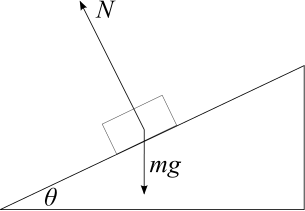
\includegraphics[width=5cm]{../../../figures/CircularMotion_d.eps}
\caption{}
\label{fig:CircularMotion_d}
\end{figure}
\\
Resolving forces vertically to find the net vertical force upwards, $F_y$:
\begin{equation*} N\cos\theta-mg=F_y \end{equation*}
and horizontally ($F_x$ acting inwards):
\begin{equation*} N\sin\theta=F_x \end{equation*}
In order for the car to travel in a circle we require $F_y=0$, since there is no vertical acceleration, and $F_x=mv^2/R$, the magnitude of the centripetal force. Therefore
\begin{equation*} N=\frac{mg}{\cos\theta} \end{equation*}
\begin{equation*} \Rightarrow N\sin\theta=mg\tan\theta=\frac{mv^2}{R} \end{equation*}
\begin{equation*} \Rightarrow v^2=gR\tan\theta \end{equation*}
So the requirement for the car to successfully go around the corner without slipping is 
\begin{equation*}
v=\sqrt{gR\tan\theta}
\end{equation*}
\\
\item With the addition of friction the diagram should look like Figure \ref{fig:CircularMotion_e}:
\begin{figure}[h]
\centering
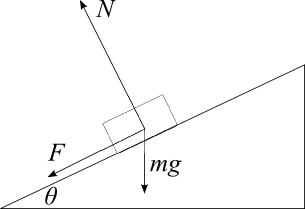
\includegraphics[width=5cm]{../../../figures/CircularMotion_e.eps}
\caption{}
\label{fig:CircularMotion_e}
\end{figure}
\\
The frictional force $\vtr{F}=\mu \vtr{N}$ at the point of slipping and has both horizontal and vertical components. Notice how it acts down the slope, since at too high a speed the car will slip up the corner, and friction always opposes the motion. Now we require
\begin{equation} \label{eq:slopeone} N\cos\theta-F\sin\theta-mg=0 \end{equation}
and
\begin{equation} \label{eq:slopetwo} N\sin\theta+F\cos\theta=\frac{mv^2}{R} \end{equation}
Substituting $F=\mu N$ in equation \eqref{eq:slopeone} gives
\begin{align*}
N\cos\theta-\mu N\sin\theta&=mg \\
\Rightarrow \frac{N\cos\theta-\mu N\sin\theta}{g}&=m
\end{align*}
then substituting in $F=\mu N$ and for $m$ (using the expression above) in equation \eqref{eq:slopetwo} we find
\begin{equation*} N\sin\theta+\mu N\cos\theta=\frac{\left(N\cos\theta-\mu N\sin\theta\right)v^2}{gR} \end{equation*} 
\begin{equation*} \Rightarrow v^2=\frac{\sin\theta+\mu \cos\theta}{\cos\theta-\mu \sin\theta}\cdot gR \end{equation*}
So now in order not to slip up the slope
\begin{equation*} v\le\sqrt{\frac{\sin\theta+\mu \cos\theta}{\cos\theta-\mu \sin\theta}\cdot gR} \end{equation*}
Notice how in the case $\theta=0$ this expression simplifies to the answer from part a), and similarly if $\mu=0$ the answer from part b) i).
\\
\item Yes there is. In this case the friction acts up the slope, as shown in Figure \ref{fig:CircularMotion_f}:
\begin{figure}[ht]
\centering
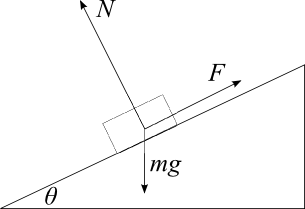
\includegraphics[width=5cm]{../../../figures/CircularMotion_f.eps}
\caption{}
\label{fig:CircularMotion_f}
\end{figure}
\\
The analysis is very similar to that in part ii), but the frictional force changes sign (since the car is now at danger of slipping down the slope). Equations \eqref{eq:slopeone} and \eqref{eq:slopetwo} become equations \eqref{eq:slopethree} and \eqref{eq:slopefour} below:
\begin{equation}
 N\cos\theta+F\sin\theta-mg=0
\label{eq:slopethree}
\end{equation}
\begin{equation} 
N\sin\theta-F\cos\theta=\frac{mv^2}{R}
\label{eq:slopefour}
\end{equation}
and the requirement for the minimum velocity becomes
\begin{equation*}
v\ge\sqrt{\frac{\sin\theta-\mu \cos\theta}{\cos\theta+\mu \sin\theta}\cdot gR}
\end{equation*}
Notice how this result is exactly the same as the one for maximum speed except $\mu$ has been replaced with $-\mu$ due to the situation being identical except for the direction of the frictional force. 
\end{enumerate}
\end{enumerate}
}
\end{problem}